 \documentclass{article}
\usepackage{tikz}
\usepackage{skak} 
\usetikzlibrary{arrows,automata}
\usetikzlibrary{positioning}

\pagestyle{empty}

\begin{document}
Bill Davis\\
Homework 6

\begin{enumerate}

\item[3.1.2]
Since the sum of the degrees of the vertices must equal 40, and there can be two vertices of degree 1, the other vertices must be of degree 2, the maximum number of vertices is $2 + \frac{38}{2} = 21$

\item[3.1.8]
a. Since n = l + i, then $i+l = mi+1$ and $l = mi+1-i$ which factors to $l=i(m-1)+1$

b. Since n = l + i, then $i+l = mi+1$ and $i-mi=l-1$ = $i(m-1) = (l-1)$ and $i=\frac{l-1}{m-1}$. And $n=m\frac{l-1}{m-1} + 1$

c. Since $n = mi+1$ and $i=\frac{n-1}{m}$ and $n=m(n-l)+1$ so $ml=nm-n+1$ and $l=\frac{mn-n+1}{m}$

\item[3.1.10]
The maximum number of vertices in a $m$-ary tree of height $h$ is $m^{h-1}+1$

\item[3.1.16]
A forest with t trees and n-vertices has n-t edges. 

\item[3.3.7]
\begin{enumerate}
\item Add 1. 2 is Closes to one, the new cycle is 1-2-1. 4 is the closest, the new cycle is 1-4-2-1, the final vertex 3 is closest to both 2 and 4. The cycle is then 1-3-4-2-1. 
\item
The final circuit is 1-4-5-3-2-6-1. 
\item
Add 1. 3 is the closest vertex, the new cycle is 1-3-1. Both 2 and 5 are 3 away from 1, add 2. The new cycle is 1-3-2-1. Next add 5, 1-3-2-5-1. Finally add 4, 1-4-3-2-5-1. 
\end{enumerate}

\item[11.A]
The Grundy function for this graph is not unique, here are two different ones. 

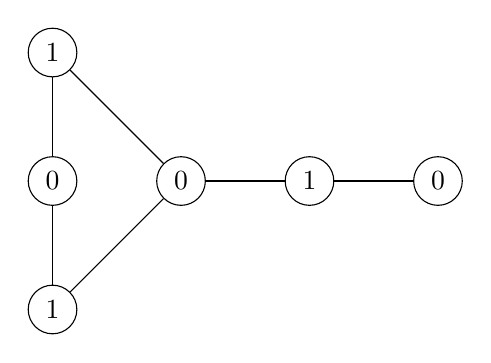
\begin{tikzpicture} [every node/.style={draw,circle}]
\node (a) {1};
\node (b) [below=of a] {0};
\node (c) [below=of b] {1};
\node (d) [right=of b] {0};
\node (e) [right=of d] {1};
\node (f) [right=of e] {0};

\draw[-](a)--(b);
\draw[-](b)--(c);
\draw[-](c)--(d);
\draw[-](d)--(a);
\draw[-](d)--(e);
\draw[-](e)--(f);
\end{tikzpicture}

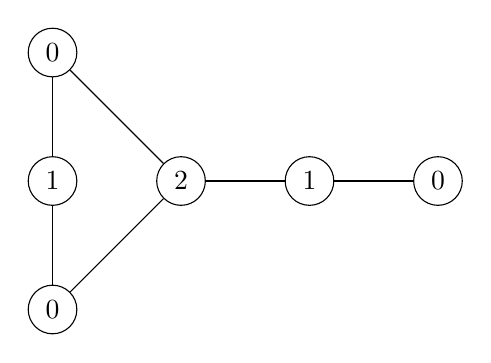
\begin{tikzpicture} [every node/.style={draw,circle}]
\node (a) {0};
\node (b) [below=of a] {1};
\node (c) [below=of b] {0};
\node (d) [right=of b] {2};
\node (e) [right=of d] {1};
\node (f) [right=of e] {0};

\draw[-](a)--(b);
\draw[-](b)--(c);
\draw[-](c)--(d);
\draw[-](d)--(a);
\draw[-](d)--(e);
\draw[-](e)--(f);
\end{tikzpicture}

\item[a]
Since there are 3 regions of degree 3 inside the circuit and 1 region of degree 5 outsite the circuit then (3-2)(3-0) + (5-2)(0-1) = 0, which means a hamilton circuit is possible 
\vspace{20 mm}

\item[b]
Since there are two regions of degree 4 inside the circuit and two regions of degree three, and one region of degree 6 outside the circuit, then (4-2)(2-0) + (3-2)(0-2) + (6-2)(0-1) = -2 a hamilton circuit is not possible for this graph. 

\end{enumerate}

\end{document}
